%!TEX root = main.tex
%=========================================================

\section{Towards Emergent Overlays}
\label{sec:overview}

\begin{figure}[t!]
	\centering
	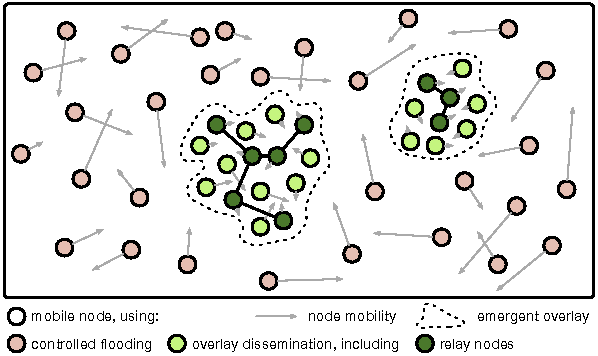
\includegraphics[scale=0.85]{figures/general_principle}
	\caption{Illustration of the general principle of emergent overlays.}
	\label{fig:general_principle}
\end{figure}

Controlled flooding is efficient when nodes density over space is small to moderate.
It is also robust in dynamic environments, as the relaying decision is based on the \emph{current} conditions during a dissemination.
However, it fails short when the density increases, leading to broadcast storm problems~\cite{BroadcastStormProblem}.
Redundant communications at the application level interfere with each other, MAC protocols require more retransmissions, leading to a chain reaction of collisions.
This quickly saturates the wireless medium, impairing reliability and increasing energy costs.
%
Overlay-based broadcast is in contrast adapted to dense environments, where a small number of well-selected relays are pre-selected and where broadcast minimizes the risk of collisions.
However, it can be ineffective when nodes are highly mobile, as maintaining the overlay would require a very frequent exchange of control messages, leading to an increase in these collisions, higher costs, and eventually lower reliability.

Human mobility behavior indicates that a hybrid approach could benefit from the resiliency and robustness of controlled flooding in general, while leveraging overlays where they are beneficial.
Mobility models~\cite{Hess:2015:DHM:2856149.2840722,Aschenbruck2009,rhee2011levy} but also large-scale measurement campaigns at large human gathering~\cite{naini2015opportunistic,versichele2012use} indicate that human users tend to aggregate around points of interest for extended periods of time.
When around these points of interests (e.g. the concert stages at the Paléo festival in~\cite{naini2015opportunistic}) the speed of users decreases or even comes to a stop.
Mobility between points of interest happens at a greater speed, and through less densely-populated areas.
%
The core contribution of this paper is the notion of \emph{emergent overlays}, illustrated by Figure~\ref{fig:general_principle}:
Nodes in a MANET use controlled flooding by default, configured for a good performance/reliability tradeoff in sparse to moderately dense areas.
Nodes in denser and more ``static'' areas (i.e. around the points of interest) \emph{autonomously} decide to switch from the controlled flooding protocol and switch to overlay-based broadcast.
%
Emergent overlays require interoperability, observation, and adaptation.

\smallskip
\noindent
\textbf{Interoperability.}
%
Broadcast messages may be emitted by any node of the network, from a zone using controlled flooding or in one using an overlay.
It is necessary that the broadcast reaches all nodes regardless of the protocols they use.
This is a problem of protocol interoperability.
Overlay-based protocols maintain efficient dissemination structure for nodes \emph{within their boundaries}.
They do not select relays for guaranteeing connectivity to nodes that do not participate to the protocol.
We develop in \S\ref{sec:mechanisms} interoperability mechanisms that properly connect and bound regions using protocols of different types, regardless of the size and shape of these regions.

\smallskip
\noindent
\textbf{Observation.}
%
Nodes must be able to reflect on their deployment environment, and evaluate in particular density and mobility.
Actively probing this information would defeat the purpose of reducing costs and improving efficiency.
Instead, we rely on passive observation that collects information from the regular operation of the broadcast and MAC protocols running on each node. 
We describe the nature and accuracy of the resulting \emph{observables} in the first part of \S\ref{sec:adaptation}.

\smallskip
\noindent
\textbf{Adaptation.}
%
The decision of when to emerge, and when to break, an emergent overlay is controlled by an adaptation policy.
Policies must be decentralized: There is no global vision of the MANET or centralized decision-making.
We only allow that specific information be piggybacked over existing messages to enable coordinated decisions between a cluster of nodes. %%% ER: remove if we do not have this in the end in the policies
The goal of the adaptation is to emerge overlays that closely correspond to dense and/or static regions, avoiding a proliferation of small and isolated overlays that could increase the cost of interoperability.
We discuss our adaptation policies in the second part of \S\ref{sec:adaptation}.

% \smallskip
% \er{keep this paragraph?}
% We note that we use counter-based controlled flooding and MPR in this paper but our results can easily be extended to other protocols of the same classes.
% Our approach may also be combined with other adaptation mechanisms that operate at the levels of the parameters of a single protocol.
% We reviews these approaches in \S\ref{sec:related}.


% \er{following text is a sketch, can be shortened and improved in style}
% Our goal is to allow nodes in a MANET to autonomously decide on the protocol that better suit their local environment.
% As the decision is local and cannot rely on a global decision-making, different nodes, or group of nodes, may choose different protocols.
% For instance, nodes in dynamic and/or sparse environments should choose to use flooding-based broadcast approaches, where the decision to forward or not an incoming message is a purely node-local decision, or to emerge an overlay with other nodes using the same protocol in their vicinity, in which case the decision of whether or not a node should forward incoming broadcast messages is decided using an overlay bootstrap procedure independent of the actual transmissions.
% We provide in this section a high-level overview of the building blocks allowing the autonomous adaptation of broadcast in MANET, and ensuring that different protocols can be used in the same system without impairing correctness or dissemination coverage.
%
% \er{%
% The goal of this section is to introduce the two next sections.
% It should be kept short and should include a figure showing the interplay between the components.
% \begin{itemize}
% 	\item nodes may use different protocols, some expect to create an overlay (e.g. pre-select which nodes are forwarders and which are not, outside of a given broadcast operation) and some will use a flooding based approach where the decision of whether or not to forward is not collective but purely individual.
% 	\item sketch the need for interoperatiliby but leave the details for the next section
% 	\item sketch the requirements for adaptation and map this to the framework presented in the previous section.
% \end{itemize}
% }
%
% \cite{one-hop-broadcast}: 2013 this study shows that broadcast within the transmission range of nodes isn't solved yet; we can use it to argue that our basic MAC protocol is used to avoid the exchange of control messages from other MAC approaches
%
%
% %
% % \begin{figure}[t]
% % 	\centering
% % 	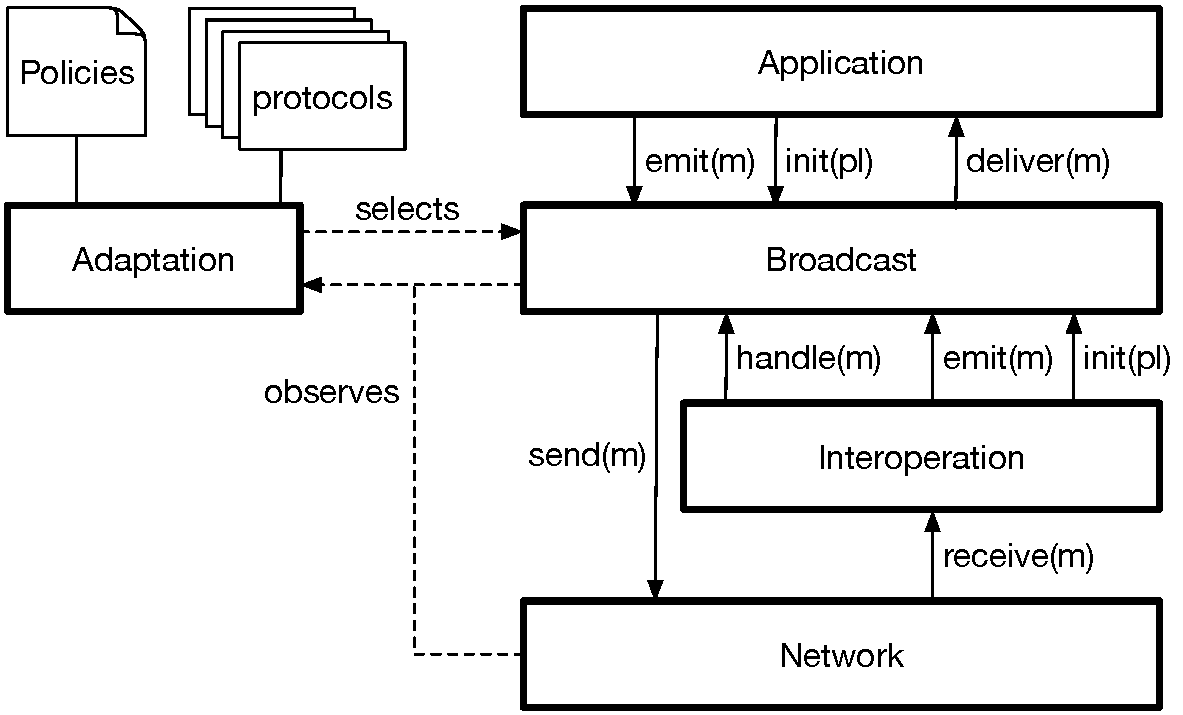
\includegraphics[scale=0.35]{figures/architecture}
% % 	\caption{System overview}
% % 	\label{fig:overview}
% % \end{figure}
%
%
% \er{recycle below}
% \subsection{Autonomous adaptation}
% \label{sec:adaptation-background}
% Adaptation refers to the ability of a system to change its behavior based on the observations of the underlaying environment.
% %
% Examples of such observables in mobile nodes are: number of nodes within broadcast areas (density), interference in signal transmissions, rate of collisions or used bandwidth.
% %
% Local information of nodes is an observable as well, such as remining battery level or nodes relatively velocity (in case a giroscope or accelerometer is available).
% %
% These observables may not be homogeneous in all nodes.
% %
% Some nodes may be positioned in densely-populated areas while others may be in sparsely-populated areas, this situation occurs in the music festival use case (as described in section~\ref{sec:introduction}).
%
% %
% We believe that there is no one-fit-all solution to broadcast in MANETs, this has been shown by priors works on adaptive schemes~\cite{hypergossiping,2001:AAR:876878.879323,adaptive_group_com_iscc02}, where a switching criterion or ~\emph{adaptation policy} is triggered to perform broadcast protocol of the same class.
% %
% Given that the operating conditions in a network are heterogeneous, adaptation policies may concern only a set of nodes.
% %
% The application of adaptive policies are based on the system observables and generally, they are applied collectively by nodes.
% %
% \raziel{Etienne: please, help me to complete/modify this next paragraph based on your draw that shows the phases of adaptation; I recall you mention a first picture where nodes run protocol A, then a phase of transition where node collectively decide to use protocol B and a third one showing some protocols running A and others running B.}
% Figure~\ref{} depict the phases of an adaptive scheme. At first, every node in the network are running a protocol $A$ (...)
%
